	This subsystem will make various queries to the database as RFID tags become ready and display
all the associated data to the Queue GUI.

\subsection{Layer Hardware}
RFID integrated readers by Chafon Technology co. This system requires the hardware to begin the process of scanning tags. The two RFID readers are attached to two 8ft speaker tripods by Pyle. The RFID readers are connected in two ways. 1st: To a 9v/3A AC adapter to supply the readers power source,  2nd: A 10ft serial connection to usb for the reader to send the data back to the server for processing the RFID tags. 

\subsection{Layer Operating System}
Windows 10 

\subsection{Layer Software Dependencies}
Chafon Technology co. provided the base C# API for the reader, modified to render tags in a readable format. 

\subsection{Subsystem 1}
This system has a single one-way interface, it parses the RFID tag from the reader into a format
that the Control system can use.

\begin{figure}[h!]
	\centering
 	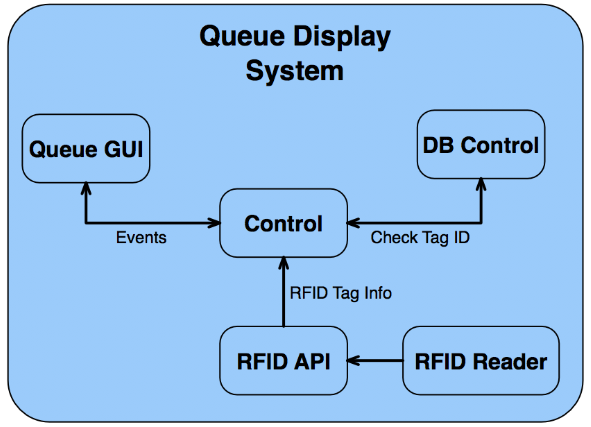
\includegraphics[width=0.60\textwidth]{images/ads_4}
 \caption{Queue Display Subsystems}
\end{figure}

\subsubsection{Subsystem Hardware}
This subsystem will identify the RFID tag that is scanned from the RFID Reader, utilizing the RFID
API it will send the data to the Control model.

\subsubsection{Subsystem Operating System}
Windows 10

\subsubsection{Subsystem Software Dependencies}
C# Chafon RFID API


\subsubsection{Subsystem Data Structures}
HTTP message once the tag id has been read is broadcast to local host. Checking the Database if the tag matches the DB will retrieve the associated data to the queue gui 




